\subsection{GKAGE} \label{results:gkage}
%In section \ref{methods} we explored three different methods for GPU accelerating existing NumPy-based code in Python: 
%1) using CuPy as a drop-in replacement for NumPy,
%2) implementing our own GPU accelerated solutions in C++ with CUDA and using pybind11 to create Python bindings for said solutions, 
%and 3) using CuPy's custom jit (just-in-time) compiled kernel support to implement kernels directly in Python, achieving similar control and granularity as with method 2.

%We chose to integrate the two following GPU accelerated functionalities into KAGE:
%1) our custom GPU accelerated hash table implemented in C++ using CUDA with pybind11 Python bindings (described in section \ref{methods:gpu_accelerating_kmer_counting}), and
%2) the CuPy drop-in solution for \textit{k}mer encoding and hashing (described in section \ref{methods:gpu_accelerating_kmer_hashing}).

%Although we also GPU accelerated the genotyping step of KAGE (described in section \ref{methods:gpu_accelerating_genotyping}) and achieved better runtimes than the original KAGE CPU implementation, an algorithmic optimization made by the KAGE developers significantly improved the runtime of the genotyping portion of KAGE.
%After having added GPU acceleration, the computation of genotype-probabilities was originally decreased from 68 down to 54 seconds, showed in table \ref{methods:integration_into_kage:tables:benchmark}.
%After benchmarking the new and optimized solution made by the KAGE developers, we found that the new runtime on the same system was 44 seconds, using the CPU.
%This optimization was made by the KAGE developers inbetween our benchmarking of the GPU accelerated genotyping step and the release of GKAGE.
%The GPU accelerated functionality implemented for the genotyping step was therefore not included in GKAGE, as it did not result in faster runtimes.

%We integrated the solutions into KAGE in such a way that the same piece of software could be run on both the CPU and the GPU.
%In fact, running GKAGE is achieved by running KAGE, using the -g flag to enable GPU acceleration.
%KAGE (and GKAGE) can be found at \url{https://github.com/kage-genotyper}.

As part of this master's project, we also present GKAGE: a new and improved version of KAGE that utilizes CUDA enabled GPUs to significantly reduce the runtime of genotyping.
As shown in section \ref{results:benchmarking:final_runtimes}, GKAGE outperforms KAGE up to 5X on a high-end compute server and 11X on a consumer grade desktop computer in terms of runtime, while producing identical outputs.
Since KAGE recently showed that it was an order of magnitude faster than any other known genotyping tool, to the best of our knowledge, GKAGE is now the fastest existing method to genotype an individual.
Additionally, GKAGE can run on commercial hardware, requiring less than 4GB of GPU memory.
KAGE (and GKAGE) can be found at \url{https://github.com/kage-genotyper}.

The final KAGE pipeline with GPU acceleration integrated can be seen in figure \ref{results:gkage:figures:gkage} below.

\begin{figure}[H]
\begin{center}
\scalebox{1}{
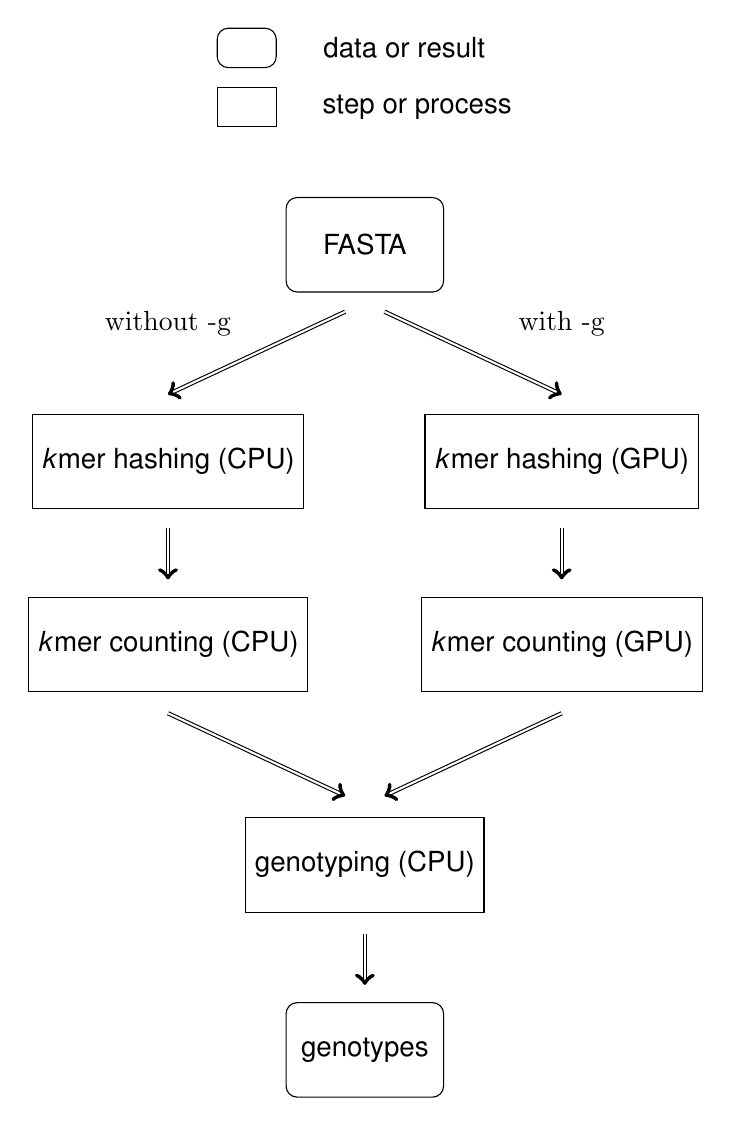
\begin{tikzpicture}
  % Hints 
  \node at(-1.5,2.5)[draw,minimum width=.75cm,minimum height=.5cm,rounded corners](){};
  \node at(.5,2.5)[](){\fontfamily{phv}\selectfont data or result};
  \node at(-1.5,1.75)[draw,minimum width=.75cm,minimum height=.5cm](){};
  \node at(.6635,1.75)[](){\fontfamily{phv}\selectfont step or process};
  \node at(0,0)[draw,minimum width=2cm,minimum height=1.2cm,rounded corners](){\fontfamily{phv}\selectfont\smaller{FASTA}};
  \node at(-2.5,-1)[](){\smaller{without -g}};
  \node at(2.5,-1)[](){\smaller{with -g}};
  \draw [double distance=.75pt,->](.25,-.85) -- (2.5,-1.9);
  \draw [double distance=.75pt,->](-.25,-.85) -- (-2.5,-1.9);
  \node at(-2.5,-2.75)[draw,minimum width=2cm,minimum height=1.2cm](){\fontfamily{phv}\selectfont\smaller{\textit{k}mer hashing (CPU)}};
  \node at(2.5,-2.75)[draw,minimum width=2cm,minimum height=1.2cm](){\fontfamily{phv}\selectfont\smaller{\textit{k}mer hashing (GPU)}};
  \draw [double distance=.75pt,->](2.5,-3.6) -- (2.5,-4.25);
  \draw [double distance=.75pt,->](-2.5,-3.6) -- (-2.5,-4.25);
  \node at(-2.5,-5.075)[draw,minimum width=2cm,minimum height=1.2cm](){\fontfamily{phv}\selectfont\smaller{\textit{k}mer counting (CPU)}};
  \node at(2.5,-5.075)[draw,minimum width=2cm,minimum height=1.2cm](){\fontfamily{phv}\selectfont\smaller{\textit{k}mer counting (GPU)}};
  \draw [double distance=.75pt,->](2.5,-5.95) -- (.25,-7);
  \draw [double distance=.75pt,->](-2.5,-5.95) -- (-.25,-7);
  \node at(0,-7.875)[draw,minimum width=2cm,minimum height=1.2cm](){\fontfamily{phv}\selectfont\smaller{genotyping (CPU)}};
  \draw [double distance=.75pt,->](0,-8.75) -- (0,-9.4);
  \node at(0,-10.225)[draw,minimum width=2cm,minimum height=1.2cm,rounded corners](){\fontfamily{phv}\selectfont\smaller{genotypes}};
\end{tikzpicture}
}
\caption{
  To run GKAGE, you simply run KAGE with the -g flag to indicate that you want to use the GPU to accelerate the processing.
  Out of the three components that we explored to GPU accelerate, only two made it into GKAGE.
  Thus, only \textit{k}mer (encoding and) hashing and \textit{k}mer counting is GPU accelerated when running KGAKE.
  The genotyping step, which constitutes a small portion of the runtime even on the CPU, is identical and runs on the CPU in both KAGE and GKAGE.
}
\label{results:gkage:figures:gkage}
\end{center}
\end{figure}
